\documentclass[12pt]{article}
\usepackage[utf8x]{inputenc}
\usepackage[spanish]{babel}
\usepackage{amsmath,amsthm}
\usepackage{graphicx}
\usepackage{url}
\usepackage[pdftex,pagebackref]{hyperref}

\newtheorem*{TD}{Teorema de Desargues}
\theoremstyle{definition}
\newtheorem{defin}{Definición}

\begin{document}
\thispagestyle{empty}
 %   Asesoren, si ceno pasa, pone Cisneros esa
%   Asesoren, si caza Cisneros esa
%   Asesoren, si caza Cisneros esa 
\begin{center}
\begin{LARGE}\textbf{Ratas que construyen sus laberintos}\end{LARGE}         
\end{center}
\vspace{6pt}

\begin{flushright}
\textit{Asesoren, si caza Cisneros esa}%palíndroma
\end{flushright}
\vspace{6pt}

Literatura y matemáticas, siempre ha habido un coqueteo entre ambas. Por 
ejemplo, en la obra de Borges hay múltiples referencias a conceptos matemáticos: 
en ``El Aleph'', al infinito; en ``La Biblioteca de Babel'', nuevamente al 
infinito y a la autoreferencia; en ``El Libro de Arena'', a la densidad de los 
números racionales; en `` Tlön, Uqbar, Orbis Tertius'', a los sistemas de 
numeración duodecimal y sexadecimal; por citar sólo algunas. En ocasiones la 
creación literaria ha sido comparada con las matemáticas, por ejemplo, en 
\textit{The Philosophy of composition}\footnote{Versión en español: 
\href{https://ciudadseva.com/texto/metodo-de-composicion/}{
https://ciudadseva.com/texto/metodo-de-composicion/}}, ensayo escrito por 
Edgar Allan Poe, refiriéndose a su famoso poema \textit{The Raven} escribe:
\begin{quotation}
 \textit{Consiste mi propósito en demostrar que ningún punto de la composición 
puede atribuirse a la intuición ni al azar; y que aquélla avanzó hacia su 
terminación, paso a paso, con la misma exactitud y la lógica rigurosa propias de 
un problema matemático.}
\end{quotation}
Por otro lado, es innegable que las matemáticas tienen aplicaciones en multitud 
de áreas y la literatura no es una excepción.
Existe un tipo de literatura en la cual las matemáticas juegan un papel 
importante en la creación literaria: la literatura potencial. Este término fue 
acuñado por el \textit{Ouvroir de Littérature Potentielle}\footnote{Que 
generalmente se traduce como ``Taller de Literatura Potencial''}, generalmente 
designado por su acrónimo \textbf{Oulipo}, el cual es una asociación fundada en 
1960 por el matemático François Le Lionnais y el escritor y poeta Raymond 
Queneau; conformada por escritores y matemáticos que, en palabras de Queneau, se 
definen como ``ratas que construyen ellas mismas el laberinto del cual se 
proponen salir''. \textbf{Oulipo} se propuso la tarea de explorar cómo las 
estructuras matemáticas pueden ser usadas en la creación literaria. La idea de 
estructura matemática se extendió para incluir cualquier tipo de escritura con 
restricciones. En su manifiesto fundacional escriben: ``Llamamos literatura 
potencial a la búsqueda de formas y de estructuras nuevas que podrán ser 
utilizadas por los escritores como mejor les parezca''. 
Además de la invención y experimentación con nuevas restricciones literarias y 
eventualmente un ejemplo de texto por cada propuesta, \textbf{Oulipo} se dedica 
a la búsqueda de quienes ellos llaman ``los plagiarios por anticipación'', 
haciendo un censo de todos los escritores que han trabajado con restricciones 
antes de la creación de \textbf{Oulipo}. Entre sus miembros se encuentran los 
escritores Italo Calvino y Georges Perec y el matemático Claude Berge, quien fue 
uno de los creadores de la moderna teoría de gráficas. Alguien se convierte en 
miembro de \textbf{Oulipo} por ``cooptación'': un nuevo miembro debe ser elegido 
unánimemente, con la condición de que jamás haya pedido ser miembro de 
\textbf{Oulipo}. Cada ``cooptado'' claramente es libre de rechazar su entrada, 
siendo su rechazo definitivo. Sin embargo, una vez elegido, no se puede 
renunciar. Los miembros continúan siendo ``oulipianos'' incluso después de su 
muerte: son entonces ``excusados por causa de deceso''.

Algunas de las restricciones literarias propuestas por \textbf{Oulipo} son las 
siguientes:
\begin{description}
 \item[Palíndroma:] palabra, número o frase que se lee igual hacia adelante que 
hacia atrás. Georges Perec escribió \textit{Le Grand Palindrome}\footnote{En 
linea en la URL palindŕomica 
\href{http://graner.net/nicolas/salocin/ten.renarg//:ptth}{
http://graner.net/nicolas/salocin/ten.renarg//:ptth}}, una palíndroma con ¡1247 
palabras! 
% Comienza y termina así: 
% \begin{quote}
% \textit{Trace l'inégal palindrome. Neige. Bagatelle, dira Hercule\dots\\[10pt]
% \dots lucre: Haridelle, ta gabegie ne mord ni la plage ni l'écart}.
% \end{quote}

\item[Lipograma:] texto en el que el escritor se impone no emplear jamás 
determinada letra, tal vez varias. Así, se encuentran prohibidas las palabras 
que contienen esa letra o esas letras. La novela \textit{La disparition}, 
también de Perec, de 300 páginas, está escrita completamente sin la letra 
``e''. (Este párrafo sólo contiene las vocales a,e,i y o).%Esta párrafo es un lipograma en ``u''.

\item[Ejercicios de Estilo:] escoger (o escribir) una historia infinitamente 
banal. La restricción consiste en escribir la misma historia varias veces, cada 
versión de la historia debe reflejar un género estilístico bien particular, de 
una lista previamente establecida o elegida al azar. Raymond Queneau escribió el 
libro titulado \textit{Exercices de style}\footnote{Extractos en francés y español en 
\href{http://arranzenfrancais.blogspot.com/2015/08/les-exercices-de-style-de-raymond.html?view=classic}{http://arranzenfrancais.blogspot.com/2015/08/les-exercices-de-style-de-raymond.html?view=classic}} en el que cuenta 99 veces la 
misma historia de formas diferentes. Esta obra fue uno de los textos precursores 
de \textbf{Oulipo}.

\item[CMMP:] esta restricción proviene del libro \textit{Cent mille milliards de 
poèmes}\footnote{Versión electrónica en 
\href{http://www.bevrowe.info/Queneau/QueneauHome\_v2.html}{
http://www.bevrowe.info/Queneau/QueneauHome\_v2.html}} de Raymond Queneau, en el 
cual escribió diez sonetos, de catorce versos cada uno. Para componer un nuevo 
soneto (uno de los cien billones), se toma el primer verso de cualquiera de los 
diez sonetos de base. Después se toma cualquier segundo verso, y así 
sucesivamente. Como hay 10 diferentes posibilidades para cada verso, en total se 
pueden formar $10^{14}=100\ 000\ 000\ 000\ 000$ sonetos. ¡Poesía y combinatoria!

\item[Desarguesiano:] restricción basada en el Teorema de Desargues, debido al 
arquitecto francés Girard Desargues (1591-1661):
%Lo que sigue son ejercicios de estilo.

\begin{description}
 \item[Teórico.] Consideremos dos triángulos $ABC$ y$A'B'C'$ en el plano.
\begin{defin}
Los triángulos están en \textit{perspectiva desde un punto}, si las rectas que 
unen los puntos correspondientes ($AA'$, $BB'$ y $CC'$) son concurrentes.
\end{defin}

\begin{defin}
Los triángulos están en \textit{perspectiva desde una recta} si los pares 
formados por rectas correspondientes ($AB$ y $A'B'$, $CB$ y $C'B'$, $AC$ y 
$A'C'$) se cortan en puntos colineales.
\end{defin}

\begin{TD}
 Si dos triángulos están en perspectiva desde un punto, entonces están en 
perspectiva desde una recta.
\end{TD}

\item[Geométrico.] En la figura hay diez rectas y diez puntos. Cada uno de los 
puntos está sobre tres rectas. Cada una de las rectas pasa por tres puntos.

\begin{center}
 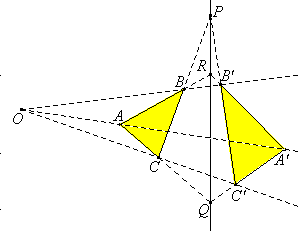
\includegraphics[height=4.5cm]{./desarg1.png}
 % desarg1.png: 301x231 pixel, 72dpi, 10.62x8.15 cm, bb=0 0 301 231
\end{center}

\item[Oulipiano.] Reemplazar figura por frase, recta por palabra y punto por 
letra. Más generalmente, reemplazar figura por texto, recta por frase y punto 
por palabra, etc.

\item[Instructivo.] Escoger diez letras. Escribir una frase de diez palabras, 
donde cada una contiene tres de las diez letras, y tal que cada una de las diez 
letras está exactamente en tres de las diez palabras.
\end{description}
\end{description}

Se puede argumentar que al dar restricciones para escribir, también se restringe 
la creatividad del autor. Los miembros de \textbf{Oulipo} piensan todo lo 
contrario, como lo expresa Georges Perec: ``Básicamente, me doy reglas para ser 
totalmente libre'' y Raymond Queneau:
\begin{quote}
 Otra idea falsa que hay actualmente, es la equivalencia que existe entre la 
inspiración, la exploración del subconsciente y la liberación; entre azar, 
automatización y libertad. Pero esta inspiración que consiste en obedecer 
ciegamente a todo impulso, es en realidad un esclavismo. El clásico que escribe 
su tragedia observando un cierto número de reglas que conoce, es más libre que 
el poeta que escribe aquello que le pasa por la cabeza, y que es esclavo de 
otras reglas que él ignora.\footnote{Le Voyage en Grèce, Gallimard, página 39.}
\end{quote}
Consideran que las restricciones formales son un poderoso estímulo para la 
imaginación. ¿Cuántas veces no nos hemos quedado sin inspiración ante una hoja 
en blanco al tener total libertad de escribir lo que queramos? El escribir con 
una restricción puede ser muy difícil, pero al mismo tiempo, como un hilo de 
Ariadna invisible, la misma restricción nos va guiando y muchas veces es más 
fácil comenzar a escribir usando lo que es permitido. La sensación de querer 
escribir algo respetando una restricción, se asemeja a tener un problema 
matemático y tratar de resolverlo, y una vez que se logra el texto uno se 
percata que se llegó a él tal y como Poe lo dice: ``con la misma exactitud y la 
lógica rigurosa propias de un problema matemático''. ¿Qué me motivó a escribir 
esto?

\begin{quotation}%Desarguesianos
\noindent Un día caluroso en la playa, Mei no cumple con el trato.\\
\textbf{Mar. Sed. Mei sin dar una red, usó uno mío.}\\[12pt]
Una sucursal del bar de moda estrena bocina francesa.\\
\textbf{Bar \textit{red led} del sur, usó una \textit{bal bon son}.}
% Afrodisiaco CUD: Canela, Uña de gato y Damiana.\\
% \textbf{Doc, fue día sin fin; con esa fea uso CUD.}
\end{quotation}
El reto de poder hacerlo y la satisfacción de haber salido del laberinto 
oulipiano, aunque el lector al leerlo, no imagine que para escribirlo, tuve que 
entrar en él.



\begin{flushright}
 José Luis Cisneros Molina\\
07/11/2010
\end{flushright}

\end{document}